\section{Simulation}
\label{sec:simulation}

The purpose of doing simulation is to have a better understanding how edge computing can
affect current mobile-cloud computing infrastructure. To put it in another way,
we ask {\em "How much better is it to offload to an edge device rather than to the cloud?"}
We focus on metrics that are important to end users, namely service time.

According to ~\cite{edgecloudsim}, the amount of time spent on WAN dominates the network delay.
Since the T1 (single-tier) model does not send tasks to the cloud, it has no WAN delay. The LAN
normally can meet user's requirment.
Figure~\ref{fig-simulation-wan} presents the average service time with 40Mpbs WAN bandwidth.
Similarly, Figure~\ref{fig-simulation-wan-4Mpbs} plots the service time while WAN only has 4Mpbs bandwidth.

It is clear that T3 has the best performance among three different computing models. Both T3 and T2 perform better
than T1 because when congestion is high, T3 and T2 can offload jobs to remote cloud. When the congestion
exceeds some threshold, T3 also has the option to offload jobs to peer edge devices.
Compare Figure~\ref{fig-simulation-wan} with Figure~\ref{fig-simulation-wan-4Mpbs}, we can find
that WAN bandwidth has little or zero effect on T1 architecture, simply because T1 does not need to offload to cloud.
With limited WAN bandwidth, both T3 and T2 has worse responsiveness. Thus it is important to maintain sufficient
bandwidth between edge devices and cloud.

{
\begin{figure}[th]
\begin{center}
	\centerline{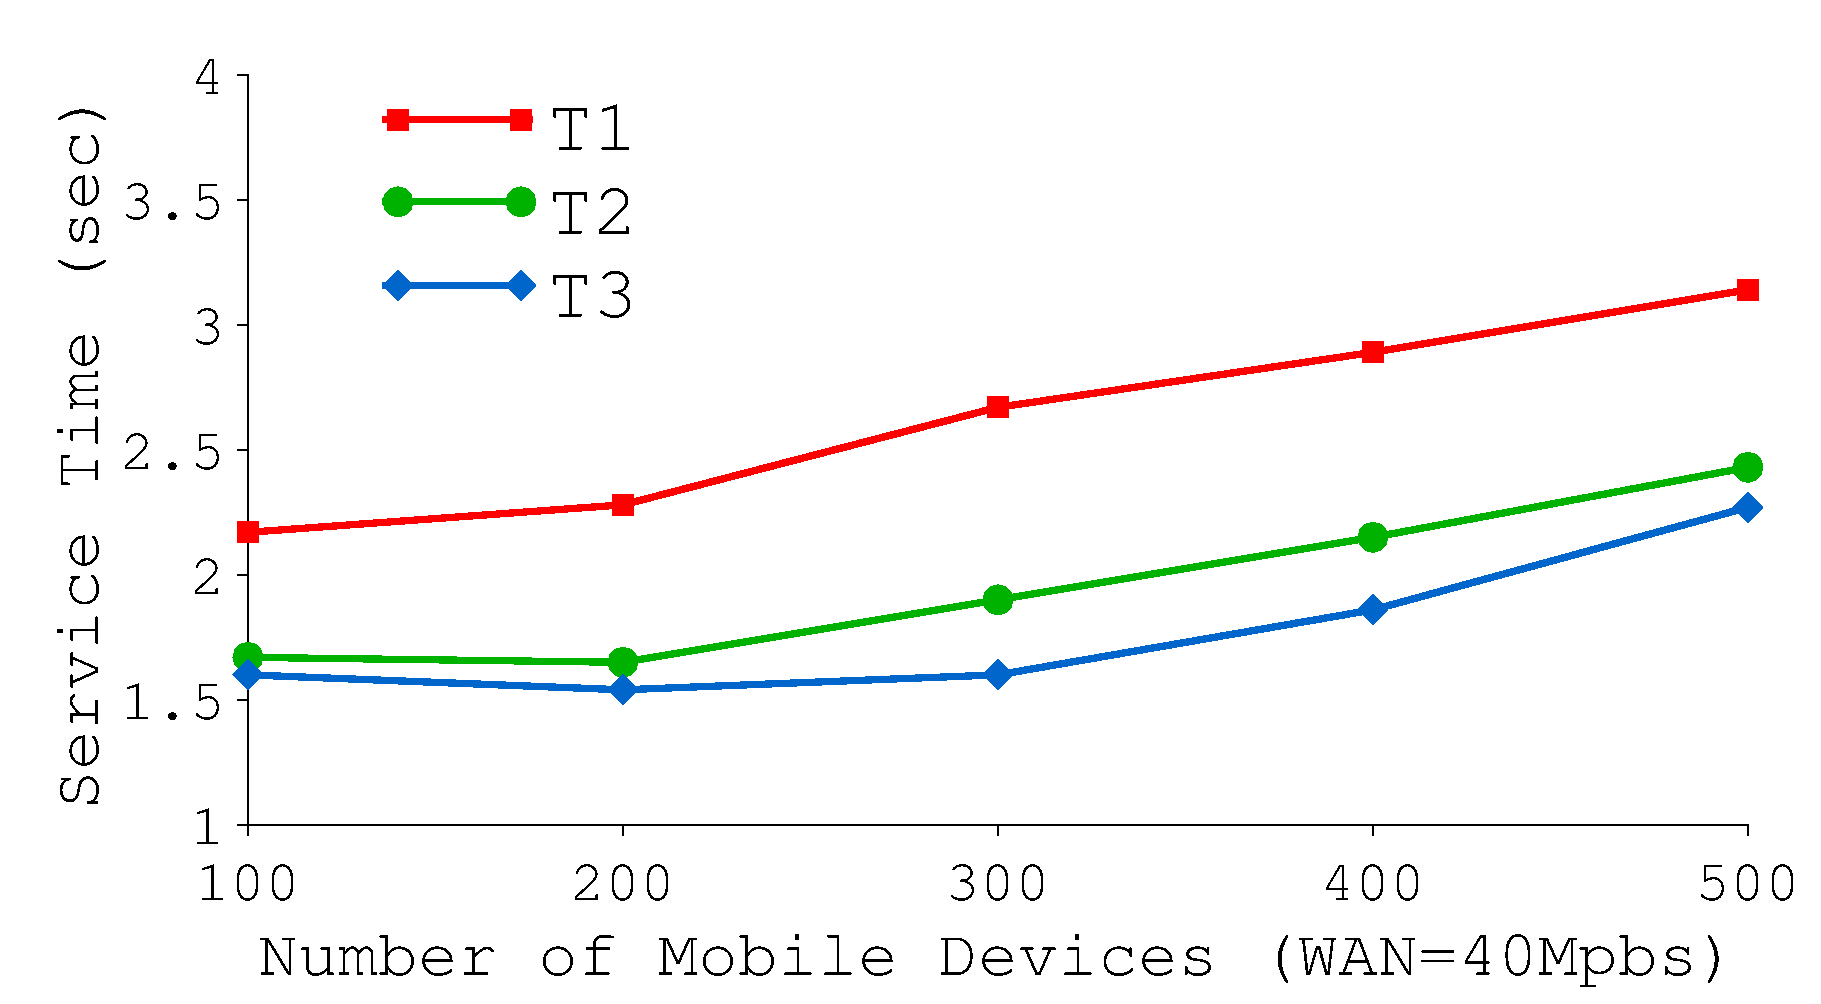
\includegraphics[width=2.5in]{Figures/g_plot_simulation-wan.pdf}}
	\mycaption{fig-simulation-wan}{Average Service Time (WAN=40Mpbs)}
	{
		T1, T2 and T3 are different computing models as described in
		Figure~\ref{fig-computing-models}. WAN bandwidth is 40Mbps,
		WLAN bandwidth is fixed 40Mbps.
	}
\end{center}
\end{figure}
}

{
\begin{figure}[th]
\begin{center}
	\centerline{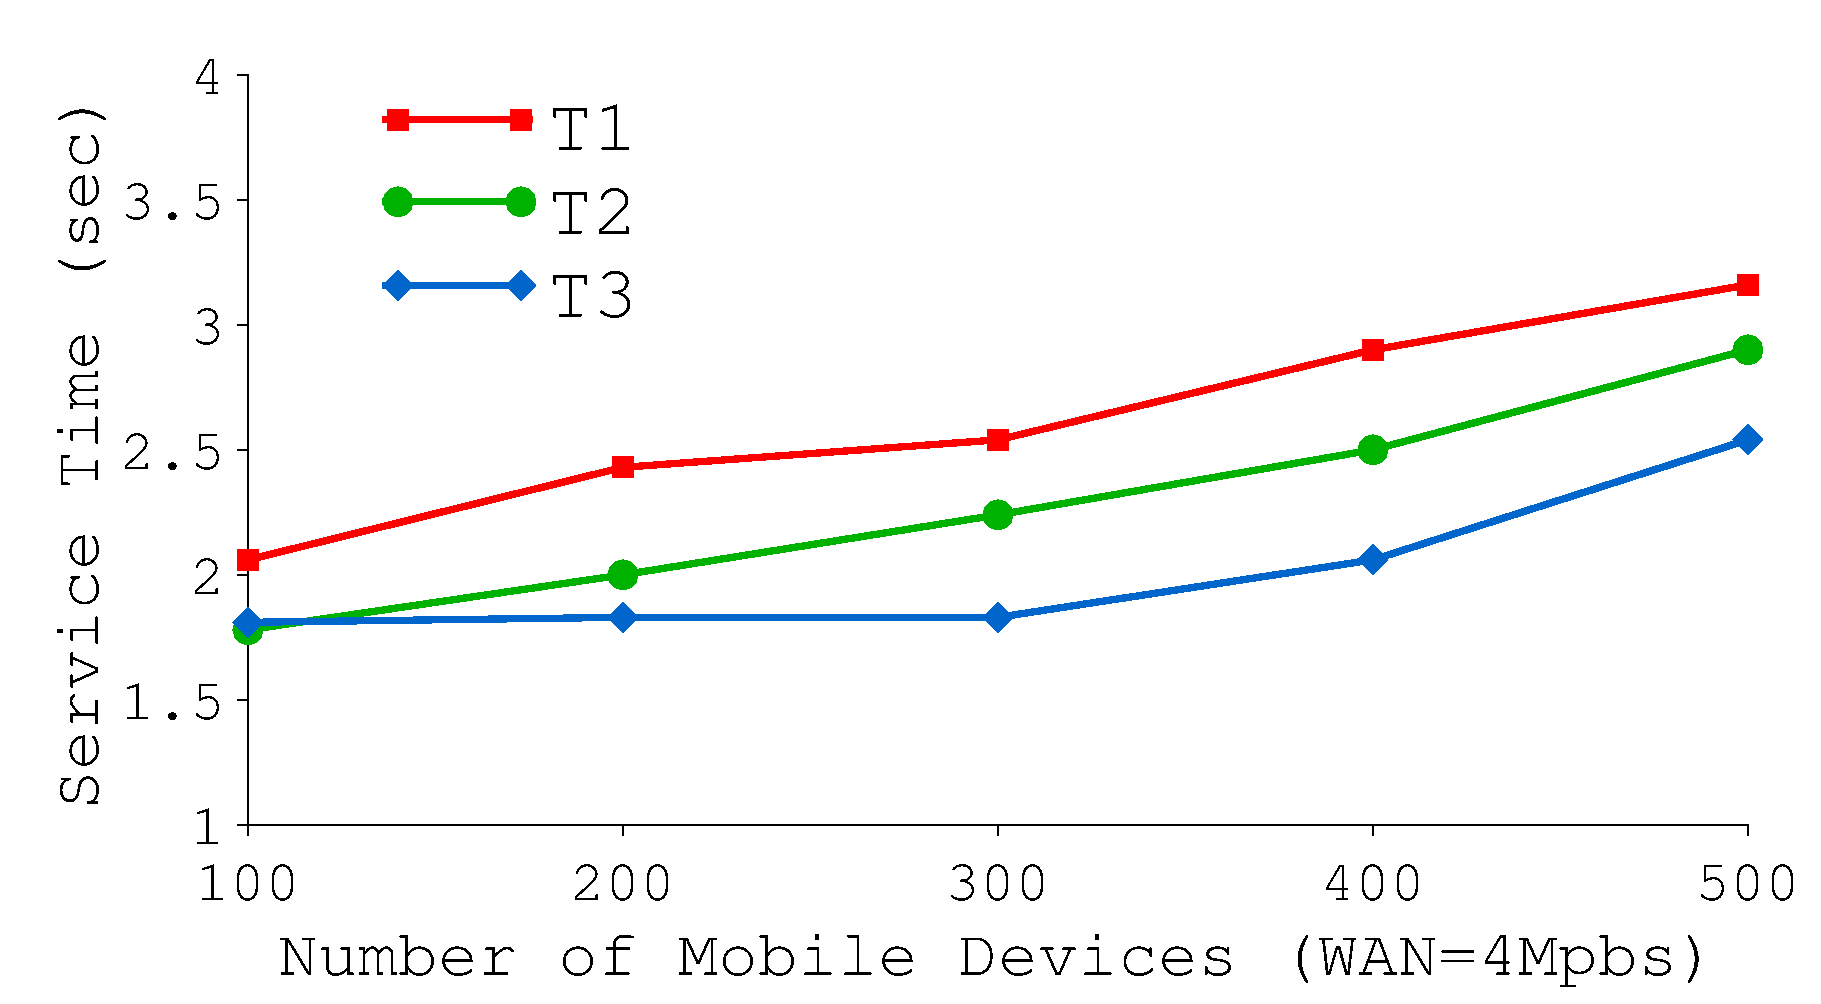
\includegraphics[width=2.5in]{Figures/g_plot_simulation-wan-4Mpbs.pdf}}
	\mycaption{fig-simulation-wan-4Mpbs}{Average Service Time (WAN=4Mpbs)}
	{
		T1, T2 and T3 are different computing models as described in
		Figure~\ref{fig-computing-models}. WAN bandwidth is 4Mbps,
		WLAN bandwidth is fixed 40Mbps.
	}
\end{center}
\end{figure}
}


\subsection{Limitation of Simulation}
Although EdgeCloudSim is able to provide average service time under different network settings and mobility settings,
the intrinsic model of using CloudSim prevents us from controlling applications in case of failures. The application
in EdgeCloudSim is described as a XML file, which lists resource (e.g., CPU, memory) requirements during runtime.
Users as us are not able to develop real applications on top of EdgeCloudSim. However, in order to achieve resilient
edge computing, we have to run mobile applications in real edge computing systems, which integrate various
fault-tolerant policies and mechanisms to provide high availability and reliability.
